\chapter{Sólidos, líquidos, gases}\label{ch:g3:solids-liquids-gases}

Uma pedra, um copo de leite, o \omterm{def:g2:air-around-us:air}{ar} de um balão: três tipos de material
que se comportam de três jeitos completamente diferentes. No ano
passado a água nos mostrou os seus três estados; neste ano descobrimos
que \emph{tudo} está em um desses três estados --- e cada estado tem
regras rigorosas.

\section{Três famílias de materiais}

Todo o material do mundo pode ser separado em três famílias, chamadas
de três \emph{estados}: \omterm{def:g3:solids-liquids-gases:solid}{sólido} como a pedra, \omterm{def:g3:solids-liquids-gases:liquid}{líquido} como o leite,
gasoso como o \omterm{def:g2:air-around-us:air}{ar}. O gelo, a água e o vapor foram o nosso primeiro
exemplo: um material visitando as três famílias. Agora vamos aprender
as regras de cada família.

\section{Os sólidos guardam o formato}

\begin{definition}[Sólido]\label{def:g3:solids-liquids-gases:solid}
Um \emph{sólido}\index{sólido} é um material que guarda o próprio
formato. Uma chave guarda o ziguezague dela no seu bolso, numa gaveta
ou debaixo d'água. Você consegue segurar um sólido entre dois dedos,
e movê-lo não muda a aparência dele. Alguns sólidos são duros
(pedra), alguns são macios (pão), alguns são flexíveis (um elástico)
--- mas, deixado em paz, cada um guarda o seu formato.
\end{definition}

\begin{example}[Um sólido feito de grãos]\label{ex:g3:solids-liquids-gases:sand}
A areia parece quebrar a regra: despejada de um balde, ela assume o
formato do montinho, quase como um \omterm{def:g3:solids-liquids-gases:liquid}{líquido}. Mas olhe de perto: a
areia é uma multidão de grãozinhos \omterm{def:g3:solids-liquids-gases:solid}{sólidos}, e \emph{cada grão} guarda
perfeitamente o seu formato. A farinha, o açúcar e o arroz fazem o
mesmo truque --- multidões de \omterm{def:g3:solids-liquids-gases:solid}{sólidos} pequenininhos que escorrem
juntos enquanto cada membro continua \omterm{def:g3:solids-liquids-gases:solid}{sólido}.
\end{example}

\section{Os líquidos escorrem --- mas guardam a quantidade}

\begin{definition}[Líquido]\label{def:g3:solids-liquids-gases:liquid}
Um \emph{líquido}\index{líquido} é um material que escorre: ele não
tem formato próprio e assume o formato do recipiente que o segura.
Mas um líquido guarda a \emph{quantidade}: despeje um copo cheio de
leite numa tigela e continua sendo a mesma quantidade de leite ---
nem uma gota a mais nem a menos, só um formato novo.
\end{definition}

\begin{omfigure}
\begin{tikzpicture}[scale=0.85]
  \draw[thick] (0,1.7) -- (0.25,0.1) -- (1.75,0.1) -- (2.0,1.7);
  \fill[omDef, opacity=0.3] (0.14,0.8) -- (1.86,0.8) -- (1.79,0.1)
    -- (0.21,0.1) -- cycle;
  \node[below, font=\small] at (1.0,-0.2) {copo};
  \draw[thick] (4.0,1.1) .. controls (4.1,0.15) .. (5.1,0.1)
    .. controls (6.1,0.15) .. (6.2,1.1);
  \fill[omDef, opacity=0.3] (4.05,0.55) .. controls (4.15,0.18)
    .. (5.1,0.14) .. controls (6.05,0.18) .. (6.15,0.55) -- cycle;
  \node[below, font=\small] at (5.1,-0.2) {tigela};
  \draw[thick] (8.2,1.7) -- (8.2,0.1) -- (11.0,0.1) -- (11.0,1.7);
  \fill[omDef, opacity=0.3] (8.2,0.45) rectangle (11.0,0.1);
  \node[below, font=\small] at (9.6,-0.2) {travessa};
  \node[above, font=\small] at (5.5,1.9)
    {o mesmo leite: formato novo a cada vez, quantidade sempre igual};
\end{tikzpicture}

{\small Um copo de leite despejado de recipiente em recipiente: o
formato obedece ao recipiente, a quantidade não obedece a ninguém.}
\end{omfigure}

\begin{proposition}[Um líquido em repouso fica na horizontal]\label{prop:g3:solids-liquids-gases:level}
A superfície de um \omterm{def:g3:solids-liquids-gases:liquid}{líquido} em repouso é sempre plana e horizontal ---
paralela ao chão. Incline a garrafa: a água lá dentro não se inclina
junto; a superfície dela continua horizontal enquanto a garrafa
pende.
\end{proposition}

\begin{omfigure}
\begin{tikzpicture}[scale=0.85]
  \draw[thick] (0.3,-0.9) rectangle (2.1,1.7);
  \fill[omDef, opacity=0.3] (0.3,-0.9) rectangle (2.1,0.5);
  \draw[omDef, very thick] (0.3,0.5) -- (2.1,0.5);
  \node[below, font=\small] at (1.2,-1.25) {em pé};
  \begin{scope}
    \clip[rotate around={-28:(6.2,0.6)}] (5.3,-0.7) rectangle (7.1,1.9);
    \fill[omDef, opacity=0.3] (4.6,-1.1) rectangle (7.8,0.5);
    \draw[omDef, very thick] (4.6,0.5) -- (7.8,0.5);
  \end{scope}
  \begin{scope}[shift={(6.2,0.6)}, rotate=-28]
    \draw[thick] (-0.9,-1.3) rectangle (0.9,1.3);
  \end{scope}
  \node[below, font=\small] at (6.2,-1.25) {inclinada: a água fica na horizontal};
\end{tikzpicture}

{\small Incline a garrafa como quiser: a superfície da água se recusa
a inclinar. Um \omterm{def:g3:solids-liquids-gases:liquid}{líquido} em repouso fica sempre na horizontal.}
\end{omfigure}

\begin{example}[O nível em ação]\label{ex:g3:solids-liquids-gases:level}
Os pedreiros usam essa lei todos os dias: o \emph{nível de bolha}
deles é uma janelinha de \omterm{def:g3:solids-liquids-gases:liquid}{líquido} com uma bolha; quando a bolha fica
entre as marcas, a prateleira está tão horizontal quanto o \omterm{def:g3:solids-liquids-gases:liquid}{líquido} lá
dentro. E, no café da manhã, observe o suco numa caixinha inclinada:
por mais que você a incline, a superfície lá dentro continua plana e
horizontal --- até encontrar o bico.
\end{example}

\section{Os gases enchem tudo}

\begin{definition}[Gás]\label{def:g3:solids-liquids-gases:gas}
Um \emph{gás}\index{gás} é um material que se espalha até ocupar
\emph{todo} o espaço que recebe. O \omterm{def:g2:air-around-us:air}{ar} é um gás: coloque-o numa
garrafa e ele enche a garrafa até o último cantinho; abra a garrafa
num cômodo maior e ele se espalha por esse cômodo também. Um gás não
tem formato próprio nem lugar próprio de descanso --- ofereça mais
espaço a ele e ele toma tudo.
\end{definition}

\begin{example}[O perfume viajante]\label{ex:g3:solids-liquids-gases:perfume}
Alguém abre um vidro de perfume numa ponta da sala. Um instante
depois, os narizes da \emph{outra} ponta percebem. O \omterm{def:g3:solids-liquids-gases:gas}{gás} do perfume
não ficou educadamente perto do vidro: solto, ele se espalhou por
todo o \omterm{def:g2:air-around-us:air}{ar} da sala, de canto a canto --- exatamente o que a família
dos gases sempre faz.
\end{example}

\begin{omfigure}
\begin{tikzpicture}[scale=0.85]
  \draw[thick] (0,0) rectangle (11,3.0);
  \draw[thick, fill=omMeth, fill opacity=0.4]
    (0.8,0) rectangle (1.4,0.9);
  \node[below, font=\small] at (1.1,-0.25) {vidro de perfume recém-aberto};
  \foreach \x/\y in {1.6/1.2, 2.1/0.6, 2.5/1.7, 3.2/1.0, 3.9/2.2,
      4.6/0.5, 5.3/1.5, 6.1/2.5, 6.9/0.9, 7.7/1.9, 8.5/0.4,
      9.2/2.3, 9.9/1.2, 10.4/2.7, 5.8/0.3, 8.9/1.4} {
    \fill[omThm, opacity=0.7] (\x,\y) circle (2.2pt);
  }
  \node[above, font=\small] at (8.3,3.1)
    {pouco depois: perfume em toda parte};
\end{tikzpicture}

{\small Um \omterm{def:g3:solids-liquids-gases:gas}{gás} solto: liberado num canto, ele se espalha até encher a
sala inteira.}
\end{omfigure}

\begin{omfigure}
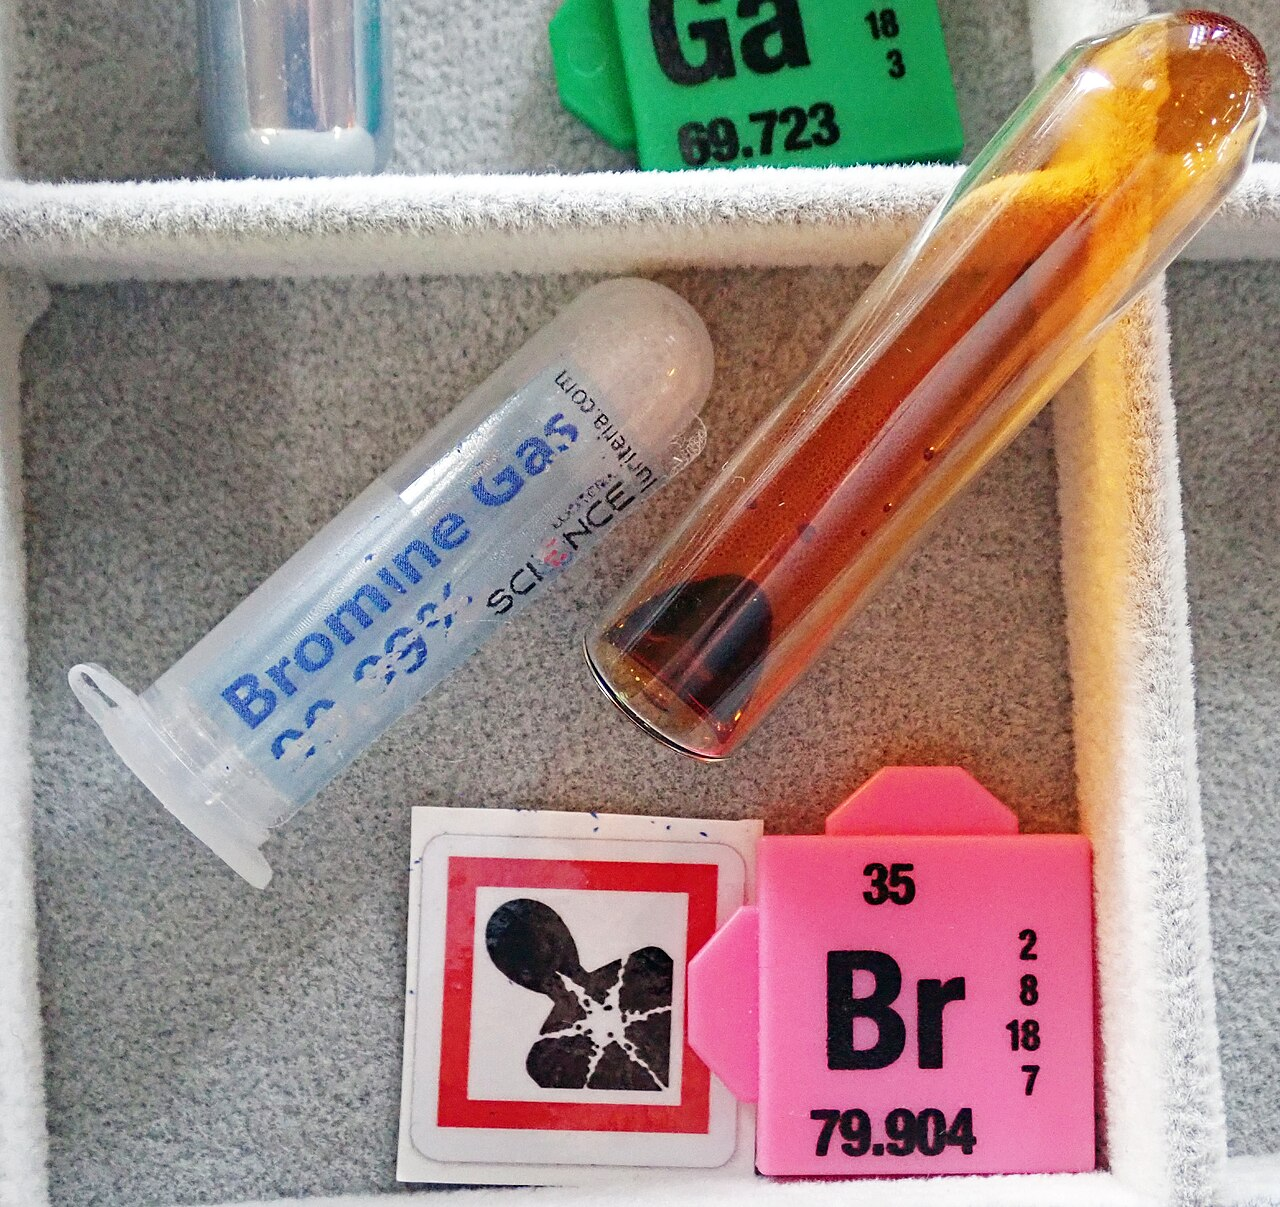
\includegraphics[width=0.4\linewidth, trim={585bp 418bp 15bp 130bp}, clip]
  {images/book1/bromine-gas.jpg}

{\small A maioria dos gases é invisível --- mas não todos. Este tubo
de vidro lacrado guarda bromo, um \omterm{def:g3:solids-liquids-gases:gas}{gás} com uma cor castanho-alaranjada
de verdade: dá para \emph{ver} o \omterm{def:g3:solids-liquids-gases:gas}{gás} enchendo cada canto do
recipiente, até encostar no vidro. \emph{Foto: James St.~John,
CC BY 2.0 (recortada).}}
\end{omfigure}

\begin{remark}[Separando os casos difíceis]\label{rem:g3:solids-liquids-gases:tricky}
Alguns materiais exigem um olhar atento. O mel escorre --- devagar,
mas escorre, assume o formato do recipiente e guarda a quantidade: é
um \omterm{def:g3:solids-liquids-gases:liquid}{líquido}, só que preguiçoso. A pasta de dente e o ketchup escorrem
quando espremidos: \omterm{def:g3:solids-liquids-gases:liquid}{líquidos} grossos. Uma esponja é um \omterm{def:g3:solids-liquids-gases:solid}{sólido} cheio de
buraquinhos com \omterm{def:g2:air-around-us:air}{ar}. E a fumaça? Partículas sólidas minúsculas
viajando num \omterm{def:g3:solids-liquids-gases:gas}{gás} quente. Na dúvida, faça as perguntas da família: ele
guarda o formato? ele escorre? ele enche todo o espaço que recebe?
\end{remark}

\section{Exercícios}

\begin{exercise}[$\star$]\label{exo:g3:solids-liquids-gases:1}
Separe nas três famílias: uma moeda; \ suco de laranja; \ o \omterm{def:g2:air-around-us:air}{ar} de um
pneu; \ uma continha de madeira; \ óleo; \ o vapor no espaço
transparente acima de uma panela fervendo.
\end{exercise}

\begin{exercise}[$\star$]\label{exo:g3:solids-liquids-gases:2}
O que um \omterm{def:g3:solids-liquids-gases:solid}{sólido} guarda e um \omterm{def:g3:solids-liquids-gases:liquid}{líquido} não guarda? O que um \omterm{def:g3:solids-liquids-gases:liquid}{líquido}
guarda quando é despejado do copo para a tigela?
\end{exercise}

\begin{exercise}[$\star$]\label{exo:g3:solids-liquids-gases:3}
Uma garrafa cheia de limonada é despejada numa saladeira larga. Agora
há mais limonada, menos ou a mesma quantidade? O que mudou?
\end{exercise}

\begin{exercise}[$\star$]\label{exo:g3:solids-liquids-gases:4}
Desenhe um aquário até a metade de água: primeiro apoiado direito,
depois inclinado sobre uma das bordas. Desenhe a superfície da água
nos dois --- como ela fica?
\end{exercise}

\begin{exercise}[$\star$]\label{exo:g3:solids-liquids-gases:5}
Como o nível de bolha de um pedreiro mostra que a prateleira está na
horizontal? Qual lei deste capítulo ele está usando?
\end{exercise}

\begin{exercise}[$\star$]\label{exo:g3:solids-liquids-gases:6}
Por que o cheiro de panqueca chega até o seu quarto lá em cima? Qual
família está trabalhando, e qual é a regra dela?
\end{exercise}

\begin{exercise}[$\star$]\label{exo:g3:solids-liquids-gases:7}
A areia escorre como um \omterm{def:g3:solids-liquids-gases:liquid}{líquido} e, mesmo assim, dizemos que ela é
sólida. Explique, usando o \cref{ex:g3:solids-liquids-gases:sand}.
\end{exercise}

\begin{exercise}[$\star$]\label{exo:g3:solids-liquids-gases:8}
O mel leva um minuto inteiro para escorrer da colher. \omterm{def:g3:solids-liquids-gases:solid}{Sólido} ou
\omterm{def:g3:solids-liquids-gases:liquid}{líquido}? Faça as perguntas da família da
\cref{rem:g3:solids-liquids-gases:tricky} e responda.
\end{exercise}

\begin{exercise}[$\star$]\label{exo:g3:solids-liquids-gases:9}
Qual família: guarda o formato próprio? \ assume o formato do
recipiente mas guarda a quantidade? \ toma todo o espaço que
consegue? Dê um membro de cada família encontrado na sua cozinha.
\end{exercise}

\begin{exercise}[$\star\star$]\label{exo:g3:solids-liquids-gases:10}
Um cubo de gelo (\omterm{def:g3:solids-liquids-gases:solid}{sólido}) \omterm{def:g2:ice-water-steam:meltfreeze}{derrete} e vira água (\omterm{def:g3:solids-liquids-gases:liquid}{líquido}), que o sol de
verão seca até virar água voadora invisível (\omterm{def:g3:solids-liquids-gases:gas}{gás}). Qual regra da
família se quebra em cada passo: o que o material deixa de guardar
quando o gelo \omterm{def:g2:ice-water-steam:meltfreeze}{derrete}? e quando a água \omterm{def:g2:ice-water-steam:evapcond}{evapora}?
\end{exercise}

\begin{exercise}[$\star\star$]\label{exo:g3:solids-liquids-gases:11}
Um balão é enchido e amarrado. Mira diz que o \omterm{def:g2:air-around-us:air}{ar} lá dentro está ``com
formato de balão, então um \omterm{def:g3:solids-liquids-gases:gas}{gás} tem formato sim''. Explique o que
está dando o formato de verdade e o que o \omterm{def:g2:air-around-us:air}{ar} faria no instante em que
o balão estourasse.
\end{exercise}
